\documentclass{article}

\usepackage[numbers,sort]{natbib}
\usepackage[czech]{babel}

\usepackage[utf8]{inputenc}
\usepackage{fancyhdr}
\usepackage{amsmath}

\usepackage[left=2cm,right=2cm,top=2.5cm,bottom=2.5cm]{geometry}
\usepackage{graphicx}

\usepackage{pdfpages}
\usepackage{gensymb}
\usepackage{url}


\bibliographystyle{vancouver} 


\pagestyle{fancy}
\lhead{(III) Studium proudění viskózní kapaliny trubicemi kruhového průřezu}
\rhead{Vladislav Wohlrath}

\author{Vladislav Wohlrath}

\begin{document}



\begin{titlepage}
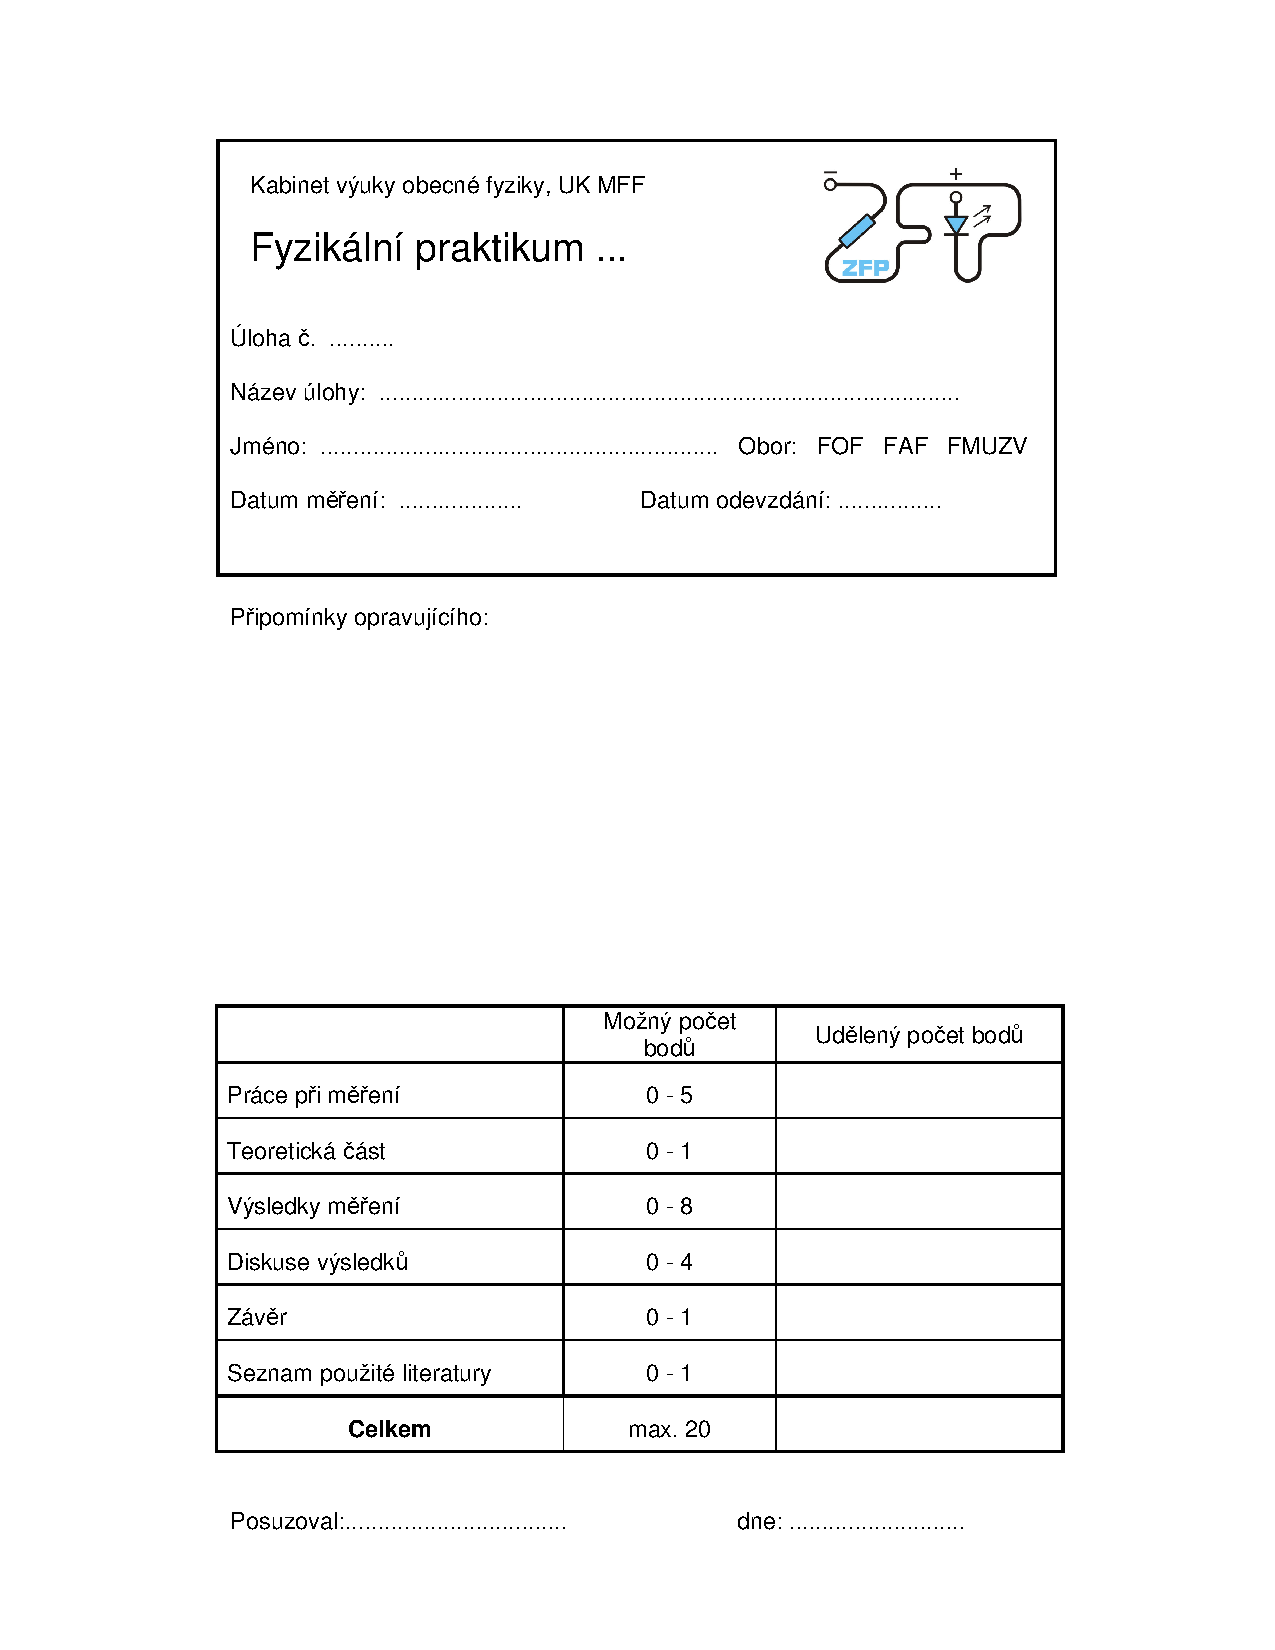
\includepdf[pages={1}]{./graficos/titlelist.pdf}
\end{titlepage}

\section*{Pracovní úkoly}
\begin{enumerate}
\item  Pro tři vodorovné trubice s různými poloměry kruhového průřezu, které jsou opatřeny manometry, změřte závislost objemového průtoku $Q_v$ na úbytku statického tlaku $\Delta p$ na vyšetřované délce trubice $l$ ve směru proudění.
\item Sestrojte graf závislosti $Q_v = Q_v (p)$.
\item Ze směrnice závislosti $Q_v = Q_v (p)$ v oblasti laminárního proudění určete poloměr trubice.
\item Upravený poloměr dosaďte do vztahů pro výpočet $Re$ a $k$.
\item Sestrojte graf závislosti $k = k(Re)$, kde k je součinitel odporu trubice a $Re$ je Reynoldsovo číslo. Do grafu vyneste teoretickou závislost pro laminární i turbulentní proudění.
\end{enumerate}




%Teoretická část
\section*{Teoretická část}

K pokusu používáme aparaturu znázorněnou na obrázku \ref{obr:zfp-nakres}. Vodorovná trubice má vnitřní poloměr $r$ a ve vzdálenosti $l$ od ústí je umístěna manometrická trubice.

\begin{figure}[h] 
\centering
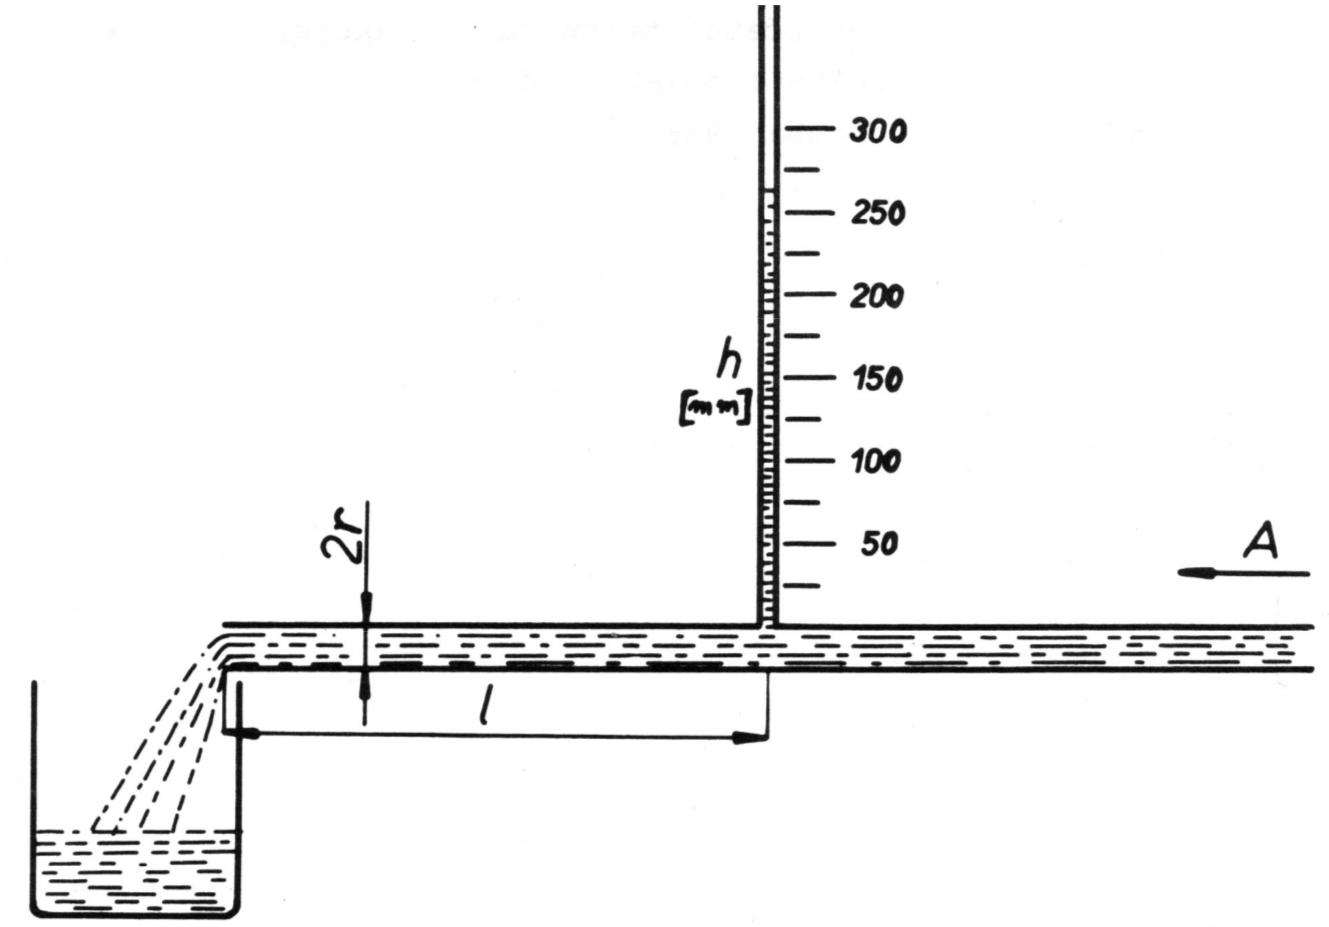
\includegraphics[width=\textwidth-2cm]{graficos/zfp}
\caption{Nákres použité aparatury (převzato z \cite{ZFP})}
\label{obr:zfp-nakres}
\end{figure}

Měříme závislost objemového průtoku $Q_v$ na úbytku statického tlaku $p$\footnote{Úbytek statického tlaku značíme $p$, zatímco $\sigma p$ značíme jeho standardní odchylku.} na délce $l$ ($Q_v=Q_v(p)$). Při určitém tlaku změříme objem vyteklé vody $V$ za dobu $t$, z toho vypočteme objemový průtok a jeho standardní odchylku podle

\begin{equation} \label{eq:Qv}
Q_v=\frac{V}{t}
\end{equation}


\begin{equation} \label{eq:chybaQv}
\sigma Q_v=Q_v \cdot \sqrt{      \left(\frac{\sigma V}{V} \right)^2+        \left(\frac{\sigma t}{t}\right)^2}
\end{equation}


Úbytek statického tlaku a jeho odchylku spočítáme z výšky vodního sloupce $h$ v manometrické trubici podle\cite{ZFP}

\begin{equation} \label{eq:tlak-na-h}
p=h\cdot \rho \cdot g
\end{equation}


\begin{equation} \label{eq:chybatlak}
\sigma p = p \cdot \sqrt{      \left(\frac{\sigma h}{h} \right)^2+        \left(\frac{\sigma \rho}{\rho}\right)^2   +   \left(\frac{\sigma g}{g}\right)^2}~,
\end{equation}
kde $\rho$ je hustota vody a $g$ je tíhové zrychlení.


Při laminárním proudění teoreticky objemový průtok závisí lineárně na úbytku tlaku, tento vztah je dán  \mbox{Poisseuillovou} rovnicí\cite{ZFP}

\begin{equation} \label{eq:poiss}
Q_v=\frac{\pi r^4}{8 \eta l} p~,
\end{equation}
kde $\eta$ je dynamická viskozita vody.

Nafitujeme tuto závislost v oblasti laminárního proudění pro každou trubici funkcí

\begin{equation} \label{eq:fit}
Q_v = a\cdot p + b
\end{equation}

Porovnáním s \eqref{eq:poiss} dostáváme

\begin{equation} \label{eq:polomer_z_a}
r=\sqrt[ 4]{\frac{8 a \eta l}{\pi}}
\end{equation}

\begin{equation}
\sigma r = \frac{1}{16} \cdot r \cdot \sqrt{      \left(\frac{\sigma a}{a} \right)^2+        \left(\frac{\sigma \eta}{\eta}\right)^2   +   \left(\frac{\sigma l}{l}\right)^2}
\end{equation}

Parametr $b$ zavádíme kvůli systematické chybě způsobené kapilárními jevy v manometrické trubici. Výška sloupce vody v \eqref{eq:tlak-na-h} neodpovídá přesně úbytku tlaku. V jedné z trubic dosahovala výška sloupce při nulovém průtoku až 1~cm.



K rozlišení laminárního a turbulentního proudění se používá Reynoldsovo číslo definované vztahem\cite{ZFP}

\begin{equation} \label{eq:reynoldsdef}
Re=\frac{r \rho v_s}{\eta}~,
\end{equation}
kde $v_s$ je střední rychlost proudění v průřezu trubice. Zřejmě platí $Q_v=\pi r^2 v_s$. Po dosazení za $v_s$ do \eqref{eq:reynoldsdef} dostáváme Reynoldsovo číslo a jeho chybu\footnote{za $r$ dosazujeme opravený poloměr z \eqref{eq:polomer_z_a}}

\begin{equation} \label{eq:reynoldsvypocet}
Re=\frac{Q_v \cdot \rho}{r \cdot \pi \cdot \eta}
\end{equation}

\begin{equation} \label{eq:reynoldschyba}
\sigma Re=Re \cdot \sqrt{      \left(\frac{\sigma Q_v}{Q_v} \right)^2+        \left(\frac{\sigma \rho}{\rho}\right)^2+        \left(\frac{\sigma r}{r}\right)^2+        \left(\frac{\sigma \eta}{\eta}\right)^2}
\end{equation}


Pokud je hodnota Reynoldsova čísla nižší než kritická hodnota (přibližně 2000 \cite{ZFP}), jedná se o laminární proudění. V rozmezí přibližně 1000--2000 \cite{ZFP} je proudění nestabilní, to se projeví vysokým rozptylem naměřených hodnot $h$ v této oblasti. Pro hodnoty vyšší než 2000 je již proudění trvale turbulentní.

Zavedeme součinitel odporu trubice $k$ a definujeme ho vztahem\cite{ZFP}

\begin{equation} \label{eq:kdef}
p=k \cdot \frac{l}{r} \cdot \frac{1}{2} \rho v_s^2
\end{equation}

Po úpravě a dosazení za $v_s$ dostáváme

\begin{equation}\label{eq:kvypocet}
k= 2\pi^2 \cdot \frac{p \cdot r^5}{l \cdot \rho \cdot Q_v^2}
\end{equation}

\begin{equation}\label{eq:kchyba}
\sigma k = k \cdot \sqrt{      \left(\frac{\sigma p}{p} \right)^2+        \left(5\frac{\sigma r}{r}\right)^2+        \left(\frac{\sigma l}{l}\right)^2+        \left(\frac{\sigma \rho}{\rho}\right)^2  +      \left(2\frac{\sigma Q_v}{Q_v}\right)^2}
\end{equation}

Porovnáním \eqref{eq:poiss}, \eqref{eq:kdef} a \eqref{eq:reynoldsdef} dostaneme pro laminární proudění

\begin{equation}\label{eq:klaminarni}
k=\frac{16}{Re}
\end{equation}

Pro turbulentní proudění se uvádí experimentálně zjistěná závislost\cite{ZFP}

\begin{equation}\label{eq:kturbulentni}
k \approx \frac{0,133}{\sqrt[4]{Re}}
\end{equation}










\section*{Podmínky a měřící přístroje}
Teplotu vody jsme změřili rtuťovým teploměrem. Vzhledem k možnému chladnutí vody během průběhu experimentu odhadujeme standardní odchylku na $1 ~\degree C$. Teplota vody byla tedy $(27 \pm 1)~ \degree C$.

Dynamická viskozita vody je při této teplotě $\eta = (0,85 ~ \pm ~0,05)~ mPa . s$ \cite{viskozita}.

Hustota vody je při této teplotě $\rho = (996~\pm~5) \cdot kg.m^{-3}$ \cite{viskozita}.

Tíhové zrychlení v Praze zaokrouhlíme na $g=(9,81 \pm 0.01) \cdot \text{m.s \textsuperscript{-2}}$ \cite{tihovyzrychleni}.

Výšku sloupce vody v manometrické trubici jsme měřili pravítkem s nejmenším dílkem $1 ~\text{mm}$. Standardní odchylku výšky sloupce odhadujeme v případě, kdy hladina nekolísá, na $\sigma h = 1~\text{mm}$ a v případě, kdy hladina kolísá, uvažujeme odchylku jako maximální změnu během daného měření.

Délku $l$ (viz obr. \ref{obr:zfp-nakres}) jsme měřili metrem s nejmenším dílkem 1~mm. Kvůli šířce manometrické trubice však odhadujeme standardní odchylku $\sigma l = 2~\text{mm}$.

Průměr trubic $r$ jsme měřili plastovým posuvným měřítkem, poloměr jsme určili jako polovinu průměru. Za standardní odchylku poloměru považujeme $\sigma r =$~0,1~mm.

Objem vytečené vody jsme měřili odměrnými válci s nejmenšími dílky 0,2~ml, 0,5~ml, 1~ml a 2~ml. Za standardní odchylku považujeme vždy nejmenší dílek.

Dobu výtoku jsme měřili stopkami s poslední zobrazenou číslicí odpovídající 0,1~s. Měření jsme prováděli tím způsobem, že při určitém čase na stopkách jsme se snažili odejmout odměrný válec od ústí trubice. Tento postup s sebou nese zřejmou nepřesnost, proto považuji standardní odchylku doby výtoku $\sigma t = \text{0,5~s}$. Tato odchylka je stejná pro všechny měření času.

%Výsledky měření
\section*{Výsledky měření}

Měření jsme provedli pro tři trubice (A, B, C) o různých poloměrech, viz tabulka \ref{tab:trubky}. Změřené hodnoty $h$, $V$, a $t$ a z nich pomocí \eqref{eq:tlak-na-h} a \eqref{eq:Qv} vypočteny $p$ a $Q_v$ s odchylkami podle \eqref{eq:chybatlak} a \eqref{eq:chybaQv} resp. jsou uvedeny v tabulkách \ref{tab:vysledkyA}, \ref{tab:vysledkyB} a \ref{tab:vysledkyC}. Závislost $Q_v=Q_v(p)$ je vvynesena do grafu na obrázku \ref{graf:Qv_na_p}. Nafitované hodnoty parametrů v \eqref{eq:fit} a poloměry trubic jsou uvedeny v tabulce \ref{tab:fit}, viz diskuze.


\begin{table}[htbp]
\centering
\begin{tabular}{|ccc|}
\hline trubice & $r$ [mm] & $l$ [cm] \\ \hline
 A & 1,2 $\pm$ 0,1 & 25,0 $\pm$ 0,2 \\ 
 B & 1,5 $\pm$ 0,1 & 24,8 $\pm$ 0,2 \\ 
 C & 2,4 $\pm$ 0,1 & 20,0 $\pm$ 0,2 \\ 
\hline 
\end{tabular} 
\caption{Měřené trubice, jejich poloměry $r$ a délky $l$}
\label{tab:trubky}
\end{table}

\begin{table}[htbp]
\centering
\begin{tabular}{|ccccc|}
\hline
$h$ [cm] & $V$ [ml] & $t$ [s] & $p$ [Pa] & $Q_v~$[ml.s\textsuperscript{-1}] \\ \hline
5,9 $\pm$ 0,1 & 8,0 $\pm$ 0,2 & 9 & 577 $\pm$ 11 & 0,89 $\pm$ 0,05\\ 
8,1 $\pm$ 0,1 & 9,4 $\pm$ 0,2 & 7 & 792 $\pm$ 11 & 1,34 $\pm$ 0,10 \\ 
11,0 $\pm$ 0,1 & 24,0 $\pm$ 0,5 & 14 & 1076 $\pm$ 12 & 1,71 $\pm$ 0,07 \\ 
12,0 $\pm$ 0,1 & 19,0 $\pm$ 0,5 & 10 & 1174 $\pm$ 12 & 1,90 $\pm$ 0,11 \\ 
12,8 $\pm$ 0,1 & 23,5 $\pm$ 0,5 & 12 & 1252 $\pm$ 12 & 1,96 $\pm$ 0,10 \\ 
13,8 $\pm$ 0,1 & 43 $\pm$ 1 & 20 & 1350 $\pm$ 12 & 2,15 $\pm$ 0,08 \\ 
14,8 $\pm$ 0,1 & 48 $\pm$ 1 & 20 & 1447 $\pm$ 13 & 2,40 $\pm$ 0,08 \\ 
15,8 $\pm$ 0,1 & 41 $\pm$ 1 & 16 & 1545 $\pm$ 13 & 2,56 $\pm$ 0,10 \\ 
16,9 $\pm$ 0,1 & 39 $\pm$ 1 & 14 & 1653 $\pm$ 13 & 2,79 $\pm$ 0,13 \\ 
17,8 $\pm$ 0,1 & 38 $\pm$ 1 & 13 & 1741 $\pm$ 14 & 2,92 $\pm$ 0,14 \\ 
18,8 $\pm$ 0,1 & 43 $\pm$ 1 & 14 & 1839 $\pm$ 14 & 3,07 $\pm$ 0,14 \\ 
20,0 $\pm$ 0,1 & 38 $\pm$ 1 & 12 & 1956 $\pm$ 14 & 3,17 $\pm$ 0,16 \\ 
21,1 $\pm$ 0,1 & 38 $\pm$ 1 & 11 & 2063 $\pm$ 15 & 3,45 $\pm$ 0,19 \\ 
22,1 $\pm$ 0,1 & 35 $\pm$ 1 & 10 & 2161 $\pm$ 15 & 3,50 $\pm$ 0,21 \\ 
23,4 $\pm$ 0,1 & 41 $\pm$ 1 & 11 & 2288 $\pm$ 16 & 3,73 $\pm$ 0,20 \\ 
24,9 $\pm$ 0,1 & 41 $\pm$ 1 & 10 & 2435 $\pm$ 16 & 4,10 $\pm$ 0,23 \\ 
26,4 $\pm$ 0,1 & 42 $\pm$ 1 & 10 & 2582 $\pm$ 17 & 4,20 $\pm$ 0,24 \\ \hline
\end{tabular}
\caption{Naměřené hodnoty pro trubici A}
\label{tab:vysledkyA}
\end{table}

\begin{table}[htbp]
\centering
\begin{tabular}{|ccccc|}
\hline
$h$ [cm] & $V$ [ml] & $t$ [s] & $p$ [Pa] & $Q_v~$[ml.s\textsuperscript{-1}] \\ \hline
2,5 $\pm$ 0,1 & 9,4 $\pm$ 0,2 & 7 & 244 $\pm$ 10 & 1,34 $\pm$ 0,10 \\ 
4,0 $\pm$ 0,1 & 21,5 $\pm$ 0,5 & 8 & 391 $\pm$ 10 & 2,69 $\pm$ 0,18 \\ 
5,0 $\pm$ 0,1 & 23,0 $\pm$ 0,5 & 7 & 489 $\pm$ 11 & 3,29 $\pm$ 0,25 \\ 
6,0 $\pm$ 0,1 & 39 $\pm$ 1 & 10 & 587 $\pm$ 11 & 3,90 $\pm$ 0,22 \\ 
7,3 $\pm$ 0,1 & 46 $\pm$ 1 & 10 & 714 $\pm$ 11 & 4,60 $\pm$ 0,26 \\ 
8,3 $\pm$ 0,1 & 41 $\pm$ 1 & 8 & 812 $\pm$ 11 & 5,13 $\pm$ 0,35 \\ 
9,3 $\pm$ 0,7 & 41 $\pm$ 1 & 8 & 909 $\pm$ 69 & 5,13 $\pm$ 0,35 \\ 
12 $\pm$ 3 & 48 $\pm$ 1 & 9 & 1170 $\pm$ 300 & 5,33 $\pm$ 0,32 \\ 
15 $\pm$ 2 & 49 $\pm$ 1 & 8 & 1470 $\pm$ 200 & 6,13 $\pm$ 0,40 \\ 
22,2 $\pm$ 0,4 & 176 $\pm$ 2 & 24 & 2171 $\pm$ 41 & 7,33 $\pm$ 0,18 \\ 
23,2 $\pm$ 0,2 & 182 $\pm$ 2 & 24 & 2269 $\pm$ 23 & 7,58 $\pm$ 0,18 \\ 
25,3 $\pm$ 0,2 & 228 $\pm$ 2 & 30 & 2474 $\pm$ 24 & 7,60 $\pm$ 0,15 \\ 
26,7 $\pm$ 0,2 & 194 $\pm$ 2 & 25 & 2611 $\pm$ 24 & 7,76 $\pm$ 0,18 \\  \hline
\end{tabular}
\caption{Naměřené hodnoty pro trubici B}
\label{tab:vysledkyB}
\end{table}

\begin{table}[htbp]
\centering
\begin{tabular}{|ccccc|}
\hline
$h$ [cm] & $V$ [ml] & $t$ [s] & $p$ [Pa] & $Q_v~$[ml.s\textsuperscript{-1}] \\ \hline
1,6 $\pm$ 0,1 & 8,0 $\pm$ 0,2 & 15 & 156 $\pm$ 10 & 0,53 $\pm$ 0,02 \\ 
3,5 $\pm$ 0,1 & 160 $\pm$ 2 & 30 & 342 $\pm$ 10 & 5,33 $\pm$ 0,12 \\ 
5,0 $\pm$ 0,6 & 200 $\pm$ 2 & 30 & 489 $\pm$ 59 & 6,67 $\pm$ 0,13 \\ 
6,0 $\pm$ 0,6 & 224 $\pm$ 2 & 30 & 587 $\pm$ 59 & 7,47 $\pm$ 0,15 \\ 
6,8 $\pm$ 0,6 & 194 $\pm$ 2 & 25 & 665 $\pm$ 59 & 7,76 $\pm$ 0,18 \\ 
8,0 $\pm$ 0,3 & 210 $\pm$ 2 & 25 & 782 $\pm$ 30 & 8,40 $\pm$ 0,19 \\ 
9,0 $\pm$ 0,1 & 226 $\pm$ 2 & 25 & 880 $\pm$ 11 & 9,04 $\pm$ 0,20 \\ 
10,1 $\pm$ 0,1 & 198 $\pm$ 2 & 20 & 988 $\pm$ 11 & 9,90 $\pm$ 0,27 \\ 
11,3 $\pm$ 0,1 & 208 $\pm$ 2 & 20 & 1105 $\pm$ 12 & 10,40 $\pm$ 0,28 \\ 
12,7 $\pm$ 0,1 & 226 $\pm$ 2 & 20 & 1242 $\pm$ 12 & 11,30 $\pm$ 0,30 \\ 
13,6 $\pm$ 0,1 & 212 $\pm$ 2 & 18 & 1330 $\pm$ 12 & 11,78 $\pm$ 0,35 \\ 
14,5 $\pm$ 0,1 & 206 $\pm$ 2 & 17 & 1418 $\pm$ 13 & 12,12 $\pm$ 0,38 \\ 
15,3 $\pm$ 0,1 & 228 $\pm$ 2 & 18 & 1496 $\pm$ 13 & 12,67 $\pm$ 0,37 \\ 
16,0 $\pm$ 0,1 & 196 $\pm$ 2 & 15 & 1565 $\pm$ 13 & 13,07 $\pm$ 0,46 \\   \hline
\end{tabular}
\caption{Naměřené hodnoty pro trubici C}
\label{tab:vysledkyC}
\end{table}


\begin{figure}[htbp] 
\centering
% GNUPLOT: LaTeX picture with Postscript
\begingroup
  \makeatletter
  \providecommand\color[2][]{%
    \GenericError{(gnuplot) \space\space\space\@spaces}{%
      Package color not loaded in conjunction with
      terminal option `colourtext'%
    }{See the gnuplot documentation for explanation.%
    }{Either use 'blacktext' in gnuplot or load the package
      color.sty in LaTeX.}%
    \renewcommand\color[2][]{}%
  }%
  \providecommand\includegraphics[2][]{%
    \GenericError{(gnuplot) \space\space\space\@spaces}{%
      Package graphicx or graphics not loaded%
    }{See the gnuplot documentation for explanation.%
    }{The gnuplot epslatex terminal needs graphicx.sty or graphics.sty.}%
    \renewcommand\includegraphics[2][]{}%
  }%
  \providecommand\rotatebox[2]{#2}%
  \@ifundefined{ifGPcolor}{%
    \newif\ifGPcolor
    \GPcolortrue
  }{}%
  \@ifundefined{ifGPblacktext}{%
    \newif\ifGPblacktext
    \GPblacktextfalse
  }{}%
  % define a \g@addto@macro without @ in the name:
  \let\gplgaddtomacro\g@addto@macro
  % define empty templates for all commands taking text:
  \gdef\gplbacktext{}%
  \gdef\gplfronttext{}%
  \makeatother
  \ifGPblacktext
    % no textcolor at all
    \def\colorrgb#1{}%
    \def\colorgray#1{}%
  \else
    % gray or color?
    \ifGPcolor
      \def\colorrgb#1{\color[rgb]{#1}}%
      \def\colorgray#1{\color[gray]{#1}}%
      \expandafter\def\csname LTw\endcsname{\color{white}}%
      \expandafter\def\csname LTb\endcsname{\color{black}}%
      \expandafter\def\csname LTa\endcsname{\color{black}}%
      \expandafter\def\csname LT0\endcsname{\color[rgb]{1,0,0}}%
      \expandafter\def\csname LT1\endcsname{\color[rgb]{0,1,0}}%
      \expandafter\def\csname LT2\endcsname{\color[rgb]{0,0,1}}%
      \expandafter\def\csname LT3\endcsname{\color[rgb]{1,0,1}}%
      \expandafter\def\csname LT4\endcsname{\color[rgb]{0,1,1}}%
      \expandafter\def\csname LT5\endcsname{\color[rgb]{1,1,0}}%
      \expandafter\def\csname LT6\endcsname{\color[rgb]{0,0,0}}%
      \expandafter\def\csname LT7\endcsname{\color[rgb]{1,0.3,0}}%
      \expandafter\def\csname LT8\endcsname{\color[rgb]{0.5,0.5,0.5}}%
    \else
      % gray
      \def\colorrgb#1{\color{black}}%
      \def\colorgray#1{\color[gray]{#1}}%
      \expandafter\def\csname LTw\endcsname{\color{white}}%
      \expandafter\def\csname LTb\endcsname{\color{black}}%
      \expandafter\def\csname LTa\endcsname{\color{black}}%
      \expandafter\def\csname LT0\endcsname{\color{black}}%
      \expandafter\def\csname LT1\endcsname{\color{black}}%
      \expandafter\def\csname LT2\endcsname{\color{black}}%
      \expandafter\def\csname LT3\endcsname{\color{black}}%
      \expandafter\def\csname LT4\endcsname{\color{black}}%
      \expandafter\def\csname LT5\endcsname{\color{black}}%
      \expandafter\def\csname LT6\endcsname{\color{black}}%
      \expandafter\def\csname LT7\endcsname{\color{black}}%
      \expandafter\def\csname LT8\endcsname{\color{black}}%
    \fi
  \fi
  \setlength{\unitlength}{0.0500bp}%
  \begin{picture}(10204.00,6802.00)%
    \gplgaddtomacro\gplbacktext{%
      \csname LTb\endcsname%
      \put(814,704){\makebox(0,0)[r]{\strut{} 0}}%
      \csname LTb\endcsname%
      \put(814,1537){\makebox(0,0)[r]{\strut{} 2}}%
      \csname LTb\endcsname%
      \put(814,2371){\makebox(0,0)[r]{\strut{} 4}}%
      \csname LTb\endcsname%
      \put(814,3204){\makebox(0,0)[r]{\strut{} 6}}%
      \csname LTb\endcsname%
      \put(814,4037){\makebox(0,0)[r]{\strut{} 8}}%
      \csname LTb\endcsname%
      \put(814,4870){\makebox(0,0)[r]{\strut{} 10}}%
      \csname LTb\endcsname%
      \put(814,5704){\makebox(0,0)[r]{\strut{} 12}}%
      \csname LTb\endcsname%
      \put(814,6537){\makebox(0,0)[r]{\strut{} 14}}%
      \csname LTb\endcsname%
      \put(946,484){\makebox(0,0){\strut{} 0}}%
      \csname LTb\endcsname%
      \put(2423,484){\makebox(0,0){\strut{} 500}}%
      \csname LTb\endcsname%
      \put(3900,484){\makebox(0,0){\strut{} 1000}}%
      \csname LTb\endcsname%
      \put(5377,484){\makebox(0,0){\strut{} 1500}}%
      \csname LTb\endcsname%
      \put(6853,484){\makebox(0,0){\strut{} 2000}}%
      \csname LTb\endcsname%
      \put(8330,484){\makebox(0,0){\strut{} 2500}}%
      \csname LTb\endcsname%
      \put(9807,484){\makebox(0,0){\strut{} 3000}}%
      \put(176,3620){\rotatebox{-270}{\makebox(0,0){\strut{}$Q_v [ml \cdot s^{-1}]$}}}%
      \put(5376,154){\makebox(0,0){\strut{}$p \text{[Pa]}$}}%
      \csname LT0\endcsname%
      \put(5377,1454){\rotatebox{10}{\makebox(0,0)[l]{\strut{}trubice A}}}%
      \csname LT1\endcsname%
      \put(2718,1954){\rotatebox{36}{\makebox(0,0)[l]{\strut{}trubice B}}}%
      \csname LT2\endcsname%
      \put(2423,4037){\rotatebox{35}{\makebox(0,0)[l]{\strut{}trubice C}}}%
    }%
    \gplgaddtomacro\gplfronttext{%
    }%
    \gplbacktext
    \put(0,0){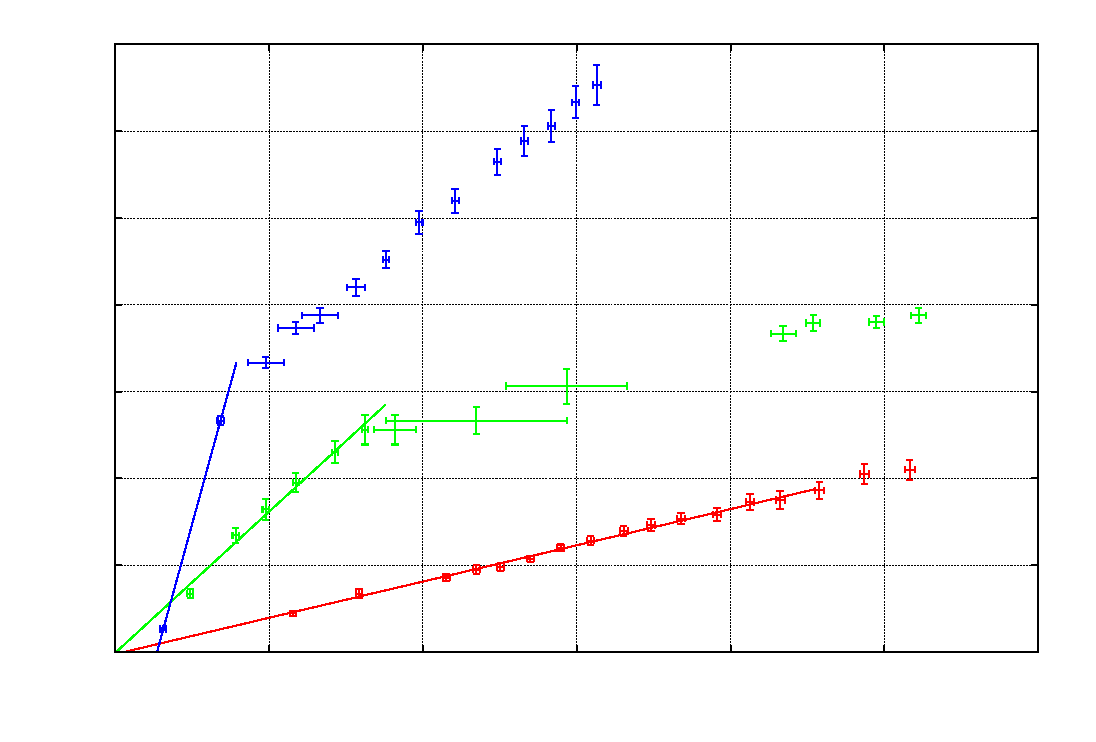
\includegraphics{graf1}}%
    \gplfronttext
  \end{picture}%
\endgroup

\caption{Závislost objemového průtoku na úbytku statického tlaku na vyšetřované délce trubice $l$}
\label{graf:Qv_na_p}
\end{figure}

\begin{table}[htbp]
\centering
\begin{tabular}{|cccc|} \hline
trubice & a [10\textsuperscript{-3}.ml.s\textsuperscript{-1}.Pa\textsuperscript{-1}] & b [ml.s\textsuperscript{-1}] & r [mm] \\ \hline
A & 1,67 $\pm$0,03  & -0,05 $\pm$ 0,05 & 0,975 $\pm$ 0,004\\ 
B & 6,508 $\pm$ 0,001 & 0,0 $\pm$ 0,3 & 1,367 $\pm$ 0,006 \\ 
C & 26 $\pm$ 5 & -3,5 $\pm$ 1,0 & 1,83 $\pm$ 0,03 \\  \hline
\end{tabular} 
\caption{Nafitované parametry $a$, $b$ a poloměry trubic}
\label{tab:fit}
\end{table}

Hodnoty $Re$ a $k$ vypočítané pomocí \eqref{eq:reynoldsvypocet} a \eqref{eq:kvypocet} a jejich odchylky pomocí \eqref{eq:reynoldschyba} a \eqref{eq:kchyba} resp. pro každé měření jsou uvedeny v tabulkách \ref{tab:kReA}, \ref{tab:kReB} a \ref{tab:kReC}. Závislost $k(Re)$ je spolu s teoretickou pro laminární \eqref{eq:klaminarni} a turbulentní \eqref{eq:kturbulentni} vynesena do grafu \ref{graf:k_na_Re}. V grafu není nakreslena jedna hodnota trubice C ($k =$~1,1).

\begin{table}[htbp]
\centering
\begin{tabular}{|cccc|}
\hline 
$p$~[Pa]  &  $Q_v$~[ml.s\textsuperscript{-1}]  & $Re$ & $k$ \\ \hline
 577 $\pm$ 11 & 0,89 $\pm$ 0,05 & 340 $\pm$ 29 & 0,051 $\pm$ 0,007\\ 
 792 $\pm$ 11 & 1,34 $\pm$ 0,10 & 514 $\pm$ 49 & 0,031 $\pm$ 0,005\\ 
 1076 $\pm$ 12 & 1,71 $\pm$ 0,07 & 656 $\pm$ 48 & 0,026 $\pm$ 0,003\\ 
 1174 $\pm$ 12 & 1,90 $\pm$ 0,11 & 727 $\pm$ 60 & 0,023 $\pm$ 0,003\\ 
 1252 $\pm$ 12 & 1,96 $\pm$ 0,10 & 749 $\pm$ 57 & 0,023 $\pm$ 0,003\\ 
 1350 $\pm$ 12 & 2,15 $\pm$ 0,08 & 822 $\pm$ 57 & 0,020 $\pm$ 0,002\\ 
 1447 $\pm$ 13 & 2,40 $\pm$ 0,08 & 918 $\pm$ 62 & 0,018 $\pm$ 0,002\\ 
 1545 $\pm$ 13 & 2,56 $\pm$ 0,10 & 980 $\pm$ 70 & 0,016 $\pm$ 0,002\\ 
 1653 $\pm$ 13 & 2,79 $\pm$ 0,13 & 1066 $\pm$ 79 & 0,015 $\pm$ 0,002\\ 
 1741 $\pm$ 14 & 2,92 $\pm$ 0,14 & 1118 $\pm$ 85 & 0,014 $\pm$ 0,002\\ 
 1839 $\pm$ 14 & 3,07 $\pm$ 0,14 & 1175 $\pm$ 86 & 0,014 $\pm$ 0,002\\ 
 1956 $\pm$ 14 & 3,17 $\pm$ 0,16 & 1211 $\pm$ 94 & 0,014 $\pm$ 0,002\\ 
 2063 $\pm$ 15 & 3,45 $\pm$ 0,19 & 1321 $\pm$ 105 & 0,012 $\pm$ 0,002\\ 
 2161 $\pm$ 15 & 3,50 $\pm$ 0,21 & 1339 $\pm$ 111 & 0,012 $\pm$ 0,002\\ 
 2288 $\pm$ 16 & 3,73 $\pm$ 0,20 & 1426 $\pm$ 112 & 0,012 $\pm$ 0,002\\ 
 2435 $\pm$ 16 & 4,10 $\pm$ 0,23 & 1568 $\pm$ 128 & 0,010 $\pm$ 0,002\\ 
 2582 $\pm$ 17 & 4,20 $\pm$ 0,24 & 1607 $\pm$ 131 & 0,010 $\pm$ 0,002\\
\hline
\end{tabular}
\caption{Hodnoty $Re$ a $k$ pro trubici A}
\label{tab:kReA}
\end{table}

\begin{table}[htbp]
\centering
\begin{tabular}{|cccc|}
\hline 
$p$~[Pa]  &  $Q_v$~[ml.s\textsuperscript{-1}]  & $Re$ & $k$ \\ \hline
 244 $\pm$ 10 & 1,34 $\pm$ 0,10 & 366 $\pm$ 35 & 0,052 $\pm$ 0,008\\ 
 391 $\pm$ 10 & 2,69 $\pm$ 0,18 & 733 $\pm$ 66 & 0,021 $\pm$ 0,003\\ 
 489 $\pm$ 11 & 3,29 $\pm$ 0,25 & 896 $\pm$ 86 & 0,015 $\pm$ 0,002\\ 
 587 $\pm$ 11 & 3,90 $\pm$ 0,22 & 1064 $\pm$ 101 & 0,015 $\pm$ 0,002\\ 
 714 $\pm$ 11 & 4,60 $\pm$ 0,26 & 1255 $\pm$ 101 & 0,013 $\pm$ 0,002\\ 
 812 $\pm$ 11 & 5,13 $\pm$ 0,35 & 1398 $\pm$ 125 & 0,012 $\pm$ 0,002\\ 
 909 $\pm$ 69 & 5,13 $\pm$ 0,35 & 1398 $\pm$ 125 & 0,013 $\pm$ 0,002\\ 
 1170 $\pm$ 300 & 5,33 $\pm$ 0,32 & 1455 $\pm$ 122 & 0,016 $\pm$ 0,005\\ 
 1470 $\pm$ 200 & 6,13 $\pm$ 0,40 & 1671 $\pm$ 148 & 0,015 $\pm$ 0,003\\ 
 2171 $\pm$ 41 & 7,33 $\pm$ 0,18 & 2001 $\pm$ 128 & 0,015 $\pm$ 0,001 \\ 
 2269 $\pm$ 23 & 7,58 $\pm$ 0,18 & 2069 $\pm$ 132 & 0,015 $\pm$ 0,001 \\ 
 2474 $\pm$ 24 & 7,60 $\pm$ 0,15 & 2073 $\pm$ 129 & 0,016 $\pm$ 0,001 \\ 
 2611 $\pm$ 24 & 7,76 $\pm$ 0,18 & 2117 $\pm$ 134 & 0,017 $\pm$ 0,001 \\ 
\hline
\end{tabular}
\caption{Hodnoty $Re$ a $k$ pro trubici B}
\label{tab:kReB}
\end{table}

\begin{table}[htbp]
\centering
\begin{tabular}{|cccc|}
\hline 
$p$~[Pa]  &  $Q_v$~[ml.s\textsuperscript{-1}]  & $Re$ & $k$ \\ \hline
 156 $\pm$ 10 & 0,53 $\pm$ 0,02 & 109 $\pm$ 8 & 1,11 $\pm$ 0,14\\ 
 342 $\pm$ 10 & 5,33 $\pm$ 0,12 & 1088 $\pm$ 70 & 0,024 $\pm$ 0,002\\ 
 489 $\pm$ 59 & 6,67 $\pm$ 0,13 & 1360 $\pm$ 87 & 0,022 $\pm$ 0,004\\ 
 587 $\pm$ 59 & 7,47 $\pm$ 0,15 & 1523 $\pm$ 97 & 0,021 $\pm$ 0,003\\ 
 665 $\pm$ 59 & 7,76 $\pm$ 0,18 & 1583 $\pm$ 102 & 0,022 $\pm$ 0,003\\ 
 782 $\pm$ 30 & 8,40 $\pm$ 0,19 & 1713 $\pm$ 111 & 0,022 $\pm$ 0,002\\ 
 880 $\pm$ 11 & 9,04 $\pm$ 0,20 & 1844 $\pm$ 119 & 0,022 $\pm$ 0,002\\ 
 988 $\pm$ 11 & 9,90 $\pm$ 0,27 & 2019 $\pm$ 134 & 0,020 $\pm$ 0,002\\ 
 1105 $\pm$ 12 & 10,40 $\pm$ 0,28 & 2121 $\pm$ 141 & 0,021 $\pm$ 0,002\\ 
 1242 $\pm$ 12 & 11,30 $\pm$ 0,30 & 2305 $\pm$ 152 & 0,020 $\pm$ 0,002\\ 
 1330 $\pm$ 12 & 11,78 $\pm$ 0,35 & 2402 $\pm$ 161 & 0,020 $\pm$ 0,002\\ 
 1418 $\pm$ 13 & 12,12 $\pm$ 0,38 & 2472 $\pm$ 168 & 0,020 $\pm$ 0,002\\ 
 1496 $\pm$ 13 & 12,67 $\pm$ 0,37 & 2584 $\pm$ 174 & 0,019 $\pm$ 0,002\\ 
 1565 $\pm$ 13 & 13,07 $\pm$ 0,46 & 2665 $\pm$ 186 & 0,019 $\pm$ 0,002\\ 
\hline
\end{tabular}
\caption{Hodnoty $k$ a $Re$ pro trubici C}
\label{tab:kReC}
\end{table}



\begin{figure}[htbp] 
\centering
% GNUPLOT: LaTeX picture with Postscript
\begingroup
  \makeatletter
  \providecommand\color[2][]{%
    \GenericError{(gnuplot) \space\space\space\@spaces}{%
      Package color not loaded in conjunction with
      terminal option `colourtext'%
    }{See the gnuplot documentation for explanation.%
    }{Either use 'blacktext' in gnuplot or load the package
      color.sty in LaTeX.}%
    \renewcommand\color[2][]{}%
  }%
  \providecommand\includegraphics[2][]{%
    \GenericError{(gnuplot) \space\space\space\@spaces}{%
      Package graphicx or graphics not loaded%
    }{See the gnuplot documentation for explanation.%
    }{The gnuplot epslatex terminal needs graphicx.sty or graphics.sty.}%
    \renewcommand\includegraphics[2][]{}%
  }%
  \providecommand\rotatebox[2]{#2}%
  \@ifundefined{ifGPcolor}{%
    \newif\ifGPcolor
    \GPcolortrue
  }{}%
  \@ifundefined{ifGPblacktext}{%
    \newif\ifGPblacktext
    \GPblacktextfalse
  }{}%
  % define a \g@addto@macro without @ in the name:
  \let\gplgaddtomacro\g@addto@macro
  % define empty templates for all commands taking text:
  \gdef\gplbacktext{}%
  \gdef\gplfronttext{}%
  \makeatother
  \ifGPblacktext
    % no textcolor at all
    \def\colorrgb#1{}%
    \def\colorgray#1{}%
  \else
    % gray or color?
    \ifGPcolor
      \def\colorrgb#1{\color[rgb]{#1}}%
      \def\colorgray#1{\color[gray]{#1}}%
      \expandafter\def\csname LTw\endcsname{\color{white}}%
      \expandafter\def\csname LTb\endcsname{\color{black}}%
      \expandafter\def\csname LTa\endcsname{\color{black}}%
      \expandafter\def\csname LT0\endcsname{\color[rgb]{1,0,0}}%
      \expandafter\def\csname LT1\endcsname{\color[rgb]{0,1,0}}%
      \expandafter\def\csname LT2\endcsname{\color[rgb]{0,0,1}}%
      \expandafter\def\csname LT3\endcsname{\color[rgb]{1,0,1}}%
      \expandafter\def\csname LT4\endcsname{\color[rgb]{0,1,1}}%
      \expandafter\def\csname LT5\endcsname{\color[rgb]{1,1,0}}%
      \expandafter\def\csname LT6\endcsname{\color[rgb]{0,0,0}}%
      \expandafter\def\csname LT7\endcsname{\color[rgb]{1,0.3,0}}%
      \expandafter\def\csname LT8\endcsname{\color[rgb]{0.5,0.5,0.5}}%
    \else
      % gray
      \def\colorrgb#1{\color{black}}%
      \def\colorgray#1{\color[gray]{#1}}%
      \expandafter\def\csname LTw\endcsname{\color{white}}%
      \expandafter\def\csname LTb\endcsname{\color{black}}%
      \expandafter\def\csname LTa\endcsname{\color{black}}%
      \expandafter\def\csname LT0\endcsname{\color{black}}%
      \expandafter\def\csname LT1\endcsname{\color{black}}%
      \expandafter\def\csname LT2\endcsname{\color{black}}%
      \expandafter\def\csname LT3\endcsname{\color{black}}%
      \expandafter\def\csname LT4\endcsname{\color{black}}%
      \expandafter\def\csname LT5\endcsname{\color{black}}%
      \expandafter\def\csname LT6\endcsname{\color{black}}%
      \expandafter\def\csname LT7\endcsname{\color{black}}%
      \expandafter\def\csname LT8\endcsname{\color{black}}%
    \fi
  \fi
  \setlength{\unitlength}{0.0500bp}%
  \begin{picture}(10204.00,6802.00)%
    \gplgaddtomacro\gplbacktext{%
      \csname LTb\endcsname%
      \put(1078,704){\makebox(0,0)[r]{\strut{} 0}}%
      \csname LTb\endcsname%
      \put(1078,1676){\makebox(0,0)[r]{\strut{} 0.01}}%
      \csname LTb\endcsname%
      \put(1078,2648){\makebox(0,0)[r]{\strut{} 0.02}}%
      \csname LTb\endcsname%
      \put(1078,3621){\makebox(0,0)[r]{\strut{} 0.03}}%
      \csname LTb\endcsname%
      \put(1078,4593){\makebox(0,0)[r]{\strut{} 0.04}}%
      \csname LTb\endcsname%
      \put(1078,5565){\makebox(0,0)[r]{\strut{} 0.05}}%
      \csname LTb\endcsname%
      \put(1078,6537){\makebox(0,0)[r]{\strut{} 0.06}}%
      \csname LTb\endcsname%
      \put(1210,484){\makebox(0,0){\strut{} 0}}%
      \csname LTb\endcsname%
      \put(2643,484){\makebox(0,0){\strut{} 500}}%
      \csname LTb\endcsname%
      \put(4076,484){\makebox(0,0){\strut{} 1000}}%
      \csname LTb\endcsname%
      \put(5509,484){\makebox(0,0){\strut{} 1500}}%
      \csname LTb\endcsname%
      \put(6941,484){\makebox(0,0){\strut{} 2000}}%
      \csname LTb\endcsname%
      \put(8374,484){\makebox(0,0){\strut{} 2500}}%
      \csname LTb\endcsname%
      \put(9807,484){\makebox(0,0){\strut{} 3000}}%
      \put(176,3620){\rotatebox{-270}{\makebox(0,0){\strut{}$k$}}}%
      \put(5508,154){\makebox(0,0){\strut{}$Re$}}%
    }%
    \gplgaddtomacro\gplfronttext{%
      \csname LTb\endcsname%
      \put(8820,6364){\makebox(0,0)[r]{\strut{}Trubice A}}%
      \csname LTb\endcsname%
      \put(8820,6144){\makebox(0,0)[r]{\strut{}Trubice B}}%
      \csname LTb\endcsname%
      \put(8820,5924){\makebox(0,0)[r]{\strut{}Trubice C}}%
      \csname LTb\endcsname%
      \put(8820,5704){\makebox(0,0)[r]{\strut{}$16/Re$}}%
      \csname LTb\endcsname%
      \put(8820,5484){\makebox(0,0)[r]{\strut{}0,133/$\sqrt[4]{Re}$}}%
    }%
    \gplbacktext
    \put(0,0){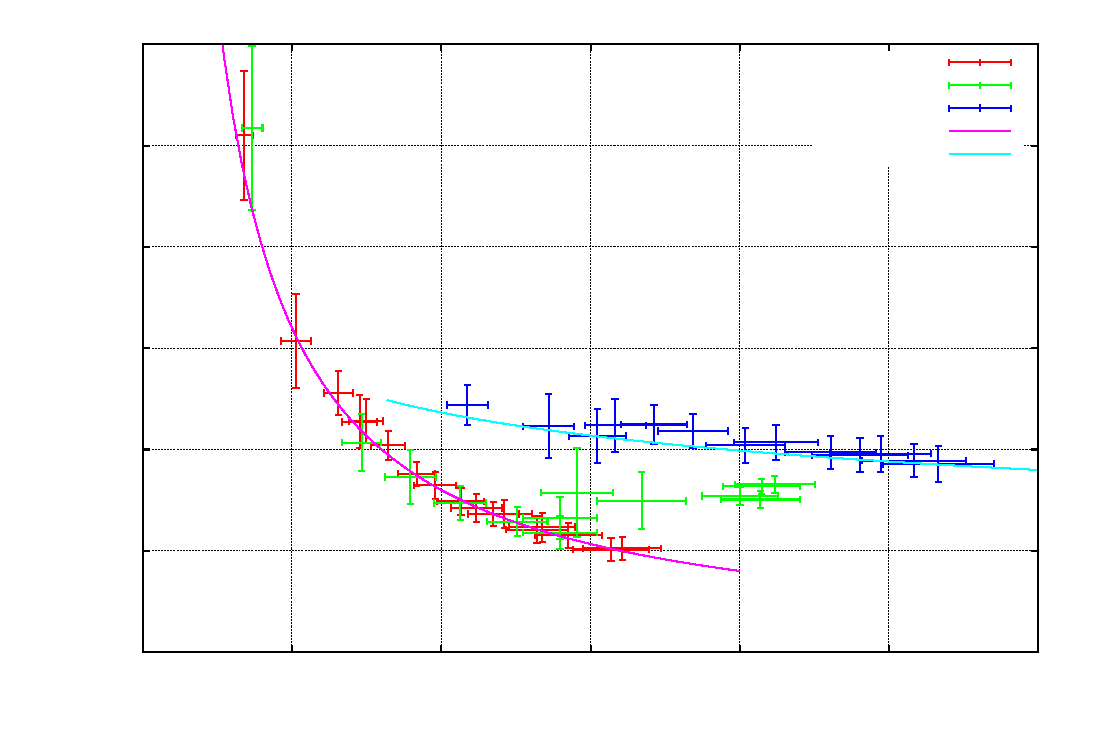
\includegraphics{grafkre}}%
    \gplfronttext
  \end{picture}%
\endgroup

\caption{Závislost součinitelu odporu trubice $k$ na Reynoldsově čísle $Re$. Zobrazeny jsou i teoretické závislosti pro laminární a turbulentní proudění.}
\label{graf:k_na_Re}
\end{figure}















%Diskuze výsledků
\section*{Diskuze}


Trubice C měla jen velmi malou oblast laminárního proudění, při výšce vodního sloupce 4,5~cm již bylo proudění nestabilní a hladina velmi kolísala. Pro velmi malé tlaky byl naopak průtok téměř neměřitelný. V oblasti laminárního proudění jsme tedy provedli jen dvě měření a při fitování závislosti \eqref{eq:fit} jsme měli k dispozici stejný počet bodů jako fitovaných parametrů. Navíc první ze dvou měření ($h =$ 1,6~cm) mohlo být zatíženo hrubou chybou, voda vytékala částečně po vnějších stěnách trubice a je možné, že se do odměrného válce nepodařila odchytit všechna. Graf \ref{graf:k_na_Re} navíc napovídá, že druhé z těchto dvou měření ($Re =$1088, $k =$ 0.024) již proběhlo při turbulentním proudění, přestože hladina v manometrické trubici ještě nekolísala. Vzhledem k těmto skutečnostem odchylku parametrů mírně nadhodnotíme a určíme s ohledem na odchylky obou bodů (viz obrázek \ref{graf:chybaC}).


\begin{figure}[htbp] 
\centering
% GNUPLOT: LaTeX picture with Postscript
\begingroup
  \makeatletter
  \providecommand\color[2][]{%
    \GenericError{(gnuplot) \space\space\space\@spaces}{%
      Package color not loaded in conjunction with
      terminal option `colourtext'%
    }{See the gnuplot documentation for explanation.%
    }{Either use 'blacktext' in gnuplot or load the package
      color.sty in LaTeX.}%
    \renewcommand\color[2][]{}%
  }%
  \providecommand\includegraphics[2][]{%
    \GenericError{(gnuplot) \space\space\space\@spaces}{%
      Package graphicx or graphics not loaded%
    }{See the gnuplot documentation for explanation.%
    }{The gnuplot epslatex terminal needs graphicx.sty or graphics.sty.}%
    \renewcommand\includegraphics[2][]{}%
  }%
  \providecommand\rotatebox[2]{#2}%
  \@ifundefined{ifGPcolor}{%
    \newif\ifGPcolor
    \GPcolortrue
  }{}%
  \@ifundefined{ifGPblacktext}{%
    \newif\ifGPblacktext
    \GPblacktextfalse
  }{}%
  % define a \g@addto@macro without @ in the name:
  \let\gplgaddtomacro\g@addto@macro
  % define empty templates for all commands taking text:
  \gdef\gplbacktext{}%
  \gdef\gplfronttext{}%
  \makeatother
  \ifGPblacktext
    % no textcolor at all
    \def\colorrgb#1{}%
    \def\colorgray#1{}%
  \else
    % gray or color?
    \ifGPcolor
      \def\colorrgb#1{\color[rgb]{#1}}%
      \def\colorgray#1{\color[gray]{#1}}%
      \expandafter\def\csname LTw\endcsname{\color{white}}%
      \expandafter\def\csname LTb\endcsname{\color{black}}%
      \expandafter\def\csname LTa\endcsname{\color{black}}%
      \expandafter\def\csname LT0\endcsname{\color[rgb]{1,0,0}}%
      \expandafter\def\csname LT1\endcsname{\color[rgb]{0,1,0}}%
      \expandafter\def\csname LT2\endcsname{\color[rgb]{0,0,1}}%
      \expandafter\def\csname LT3\endcsname{\color[rgb]{1,0,1}}%
      \expandafter\def\csname LT4\endcsname{\color[rgb]{0,1,1}}%
      \expandafter\def\csname LT5\endcsname{\color[rgb]{1,1,0}}%
      \expandafter\def\csname LT6\endcsname{\color[rgb]{0,0,0}}%
      \expandafter\def\csname LT7\endcsname{\color[rgb]{1,0.3,0}}%
      \expandafter\def\csname LT8\endcsname{\color[rgb]{0.5,0.5,0.5}}%
    \else
      % gray
      \def\colorrgb#1{\color{black}}%
      \def\colorgray#1{\color[gray]{#1}}%
      \expandafter\def\csname LTw\endcsname{\color{white}}%
      \expandafter\def\csname LTb\endcsname{\color{black}}%
      \expandafter\def\csname LTa\endcsname{\color{black}}%
      \expandafter\def\csname LT0\endcsname{\color{black}}%
      \expandafter\def\csname LT1\endcsname{\color{black}}%
      \expandafter\def\csname LT2\endcsname{\color{black}}%
      \expandafter\def\csname LT3\endcsname{\color{black}}%
      \expandafter\def\csname LT4\endcsname{\color{black}}%
      \expandafter\def\csname LT5\endcsname{\color{black}}%
      \expandafter\def\csname LT6\endcsname{\color{black}}%
      \expandafter\def\csname LT7\endcsname{\color{black}}%
      \expandafter\def\csname LT8\endcsname{\color{black}}%
    \fi
  \fi
  \setlength{\unitlength}{0.0500bp}%
  \begin{picture}(6802.00,4534.00)%
    \gplgaddtomacro\gplbacktext{%
      \csname LTb\endcsname%
      \put(682,704){\makebox(0,0)[r]{\strut{} 0}}%
      \csname LTb\endcsname%
      \put(682,1298){\makebox(0,0)[r]{\strut{} 1}}%
      \csname LTb\endcsname%
      \put(682,1892){\makebox(0,0)[r]{\strut{} 2}}%
      \csname LTb\endcsname%
      \put(682,2487){\makebox(0,0)[r]{\strut{} 3}}%
      \csname LTb\endcsname%
      \put(682,3081){\makebox(0,0)[r]{\strut{} 4}}%
      \csname LTb\endcsname%
      \put(682,3675){\makebox(0,0)[r]{\strut{} 5}}%
      \csname LTb\endcsname%
      \put(682,4269){\makebox(0,0)[r]{\strut{} 6}}%
      \csname LTb\endcsname%
      \put(814,484){\makebox(0,0){\strut{} 0}}%
      \csname LTb\endcsname%
      \put(1513,484){\makebox(0,0){\strut{} 50}}%
      \csname LTb\endcsname%
      \put(2212,484){\makebox(0,0){\strut{} 100}}%
      \csname LTb\endcsname%
      \put(2911,484){\makebox(0,0){\strut{} 150}}%
      \csname LTb\endcsname%
      \put(3610,484){\makebox(0,0){\strut{} 200}}%
      \csname LTb\endcsname%
      \put(4308,484){\makebox(0,0){\strut{} 250}}%
      \csname LTb\endcsname%
      \put(5007,484){\makebox(0,0){\strut{} 300}}%
      \csname LTb\endcsname%
      \put(5706,484){\makebox(0,0){\strut{} 350}}%
      \csname LTb\endcsname%
      \put(6405,484){\makebox(0,0){\strut{} 400}}%
      \put(176,2486){\rotatebox{-270}{\makebox(0,0){\strut{}$Q_v [ml \cdot s^{-1}]$}}}%
      \put(3609,154){\makebox(0,0){\strut{}$p \text{[Pa]}$}}%
    }%
    \gplgaddtomacro\gplfronttext{%
    }%
    \gplbacktext
    \put(0,0){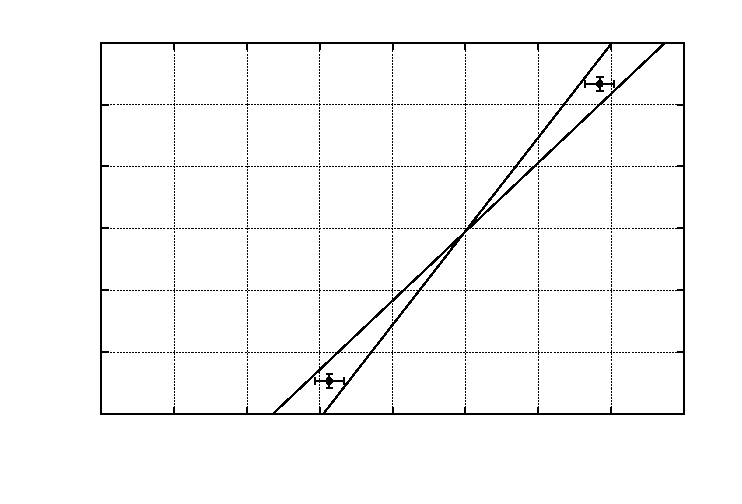
\includegraphics{grafdisk}}%
    \gplfronttext
  \end{picture}%
\endgroup

\caption{ První dva změřené body v oblasti laminárního proudění pro trubici C. Dvě přímky \mbox{$Q_v=(a+\sigma a)\cdot p+(b-\sigma b)$}, \mbox{$Q_v=(a-\sigma a)\cdot p+(b+\sigma b)$} ilustrují odhadnutou odchylku parametrů $a$ a $b$.}
\label{graf:chybaC}
\end{figure}

Opravené poloměry se s těmi naměřenými přiliš neshodují, naměřené jsou vždy vyšší. Jedním možným vysvětlením je neodhalená systematická chyba při měření posuvným měřítkem. Poloměr jsme měřili tím způsobem, že jsme dovnitř trubice strčili pacičky měřítka a roztáhli je na celý průměr trubice. Posuvné měřítko bylo plastové, takže je možné, že jsme působili přiliš velkou silou, pacičky se deformovali a naměřili jsme vyšší hodnotu.

Závislost $k(Re)$ vyšla podle očekávání. Trubice A měla nejmenší poloměr, při všech měřeních v ní voda proudila laminárně a závislost přesně odpovídá teoretické. U trubice C proběhly všechny měření kromě prvních dvou při turbulentním proudění a závislost téměř přesně odpovídá teoretické pro turbulentní proudění. V trubici B bylo nejdříve laminární proudění a přibližně při $Re=$1300 začalo být nestabilní. Pro $Re>$2000 bylo již proudění trvale turbulentní. Skutečně hodnoty $k$ nejdříve odpovídají křivce pro laminární proudění a poté se začínají blížit té pro turbulentní.

%Závěr
\section*{Závěr}

Poloměry trubic jsme určili ze směrnice závislosti objemového průtoku na úbytku statického tlaku při laminárním proudění takto:

\begin{itemize}
\item Trubice A: $r=$~(0,975$\pm$0,004)~mm 
\item Trubice B: $r=$~(1,367$\pm$0,006)~mm
\item Trubice C: $r=$~(1,83$\pm$0,03)~mm
\end{itemize}

Od hodnot změřených posuvným měřítkem se značně liší.

Ve všech trubicích začalo být proudění nestabilní při hodnotě Reynoldsova čísla přibližně 1400--1500. Pro hodnoty menší bylo laminární.


\bibliography{source}

\end{document}
